\chapter{An Oscillator in 4 Parts}
\lstset{style=6502Style}
\begin{figure}[H]
{
  \setlength{\tabcolsep}{3.0pt}
  \setlength\cmidrulewidth{\heavyrulewidth} % Make cmidrule = 
    \begin{adjustbox}{width=12cm,center}
  \begin{subfigure}{0.3\textwidth}
  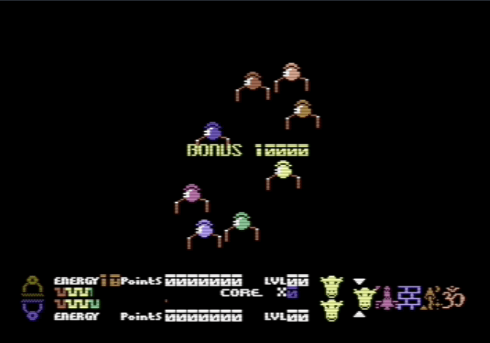
\includegraphics[width=4cm]{torus/bonusbounty.png}%
  \end{subfigure}
  \begin{subfigure}{0.3\textwidth}
  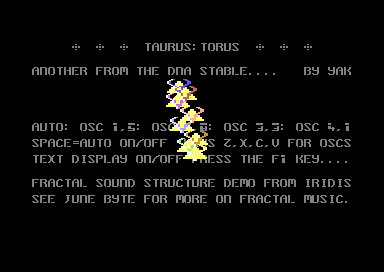
\includegraphics[width=4cm]{torus/torus.png}%
  \end{subfigure}
  \end{adjustbox}
}\caption[]{The Torus oscillator animation and Iridis' bonus animation.}
\end{figure}

The Torus demo is also the laboratory where the elegant animation used when awarding a bonus was developed. The code
handling each is identical and was only very lightly modified for the final game.

\begin{minipage}[b]{0.45\linewidth}
\centering
\CopyPartialFile{../iridisalpha/demos/torus/src/torus.asm}{tmp.asm}{361}{412}%
\lstinputlisting[caption=Animation in Torus Demo,basicstyle=\tiny]{tmp.asm}
\end{minipage}
\hspace{0.5cm}
\begin{minipage}[b]{0.45\linewidth}
\centering
\CopyPartialFile{../iridisalpha/src/iridisalpha.asm}{tmp.asm}{5055}{5106}%
\lstinputlisting[caption=... and Iridis Alpha,basicstyle=\tiny]{tmp.asm}
\end{minipage}


\begin{tcolorbox}[%
  breakable,
  parbox = false,
  frame hidden,
  sharp corners,
  after skip=10pt,
  overlay broken = {
    \draw[]
      (frame.north west) rectangle (frame.south east);},
]{}
A Testing Hack

In the CheckKeyboardInGame Routine, we find the following:
\CopyPartialFile{../iridisalpha/src/iridisalpha.asm}{tmp.asm}{7909}{7920}%
\lstinputlisting[basicstyle=\tiny]{tmp.asm}

In the above the `canAwardBonus` byte is the first letter in the name of the player with the top score in the Hi-Score table. By default this is 'YAK':
\CopyPartialFile{../iridisalpha/src/iridisalpha.asm}{tmp.asm}{8713}{8716}%
\lstinputlisting[basicstyle=\tiny]{tmp.asm}

But if we change 'Y' to \icode{\$1C} like so, we can activate the hack:

\begin{lstlisting}[basicstyle=\tiny]
hiScoreTablePtr           .TEXT "0068000"
canAwardBonus             .TEXT $1C,"AK "
\end{lstlisting}

Note that \icode{\$1C} is charset code for a bull's head symbol in Iridis Alpha, so it is also possible to enter this as the initial of a high scorer name if we get a score that puts us to the top of the table:

\CopyPartialFile{../iridisalpha/src/graphics/charset.asm}{tmp.asm}{287}{296}%
\lstinputlisting[basicstyle=\tiny]{tmp.asm}


I'm guessing this was used for testing the animation routine and left in as an Easter egg.

\end{tcolorbox}%

To start getting a handle on how the oscillation animation works, lets plot the first 24 animations that the Torus
demo uses when left to its own devices. We get a variety of different trajectories, some relatively simple, some
quite convoluted.

\clearpage
\begin{figure}[p]
    \centering
    \foreach \l in {0, ..., 23}
    {
      \begin{subfigure}{0.3\textwidth}
        \begin{tikzpicture}
        \begin{axis}[
          xmin = 0, xmax = 150,
               ymin = 0, ymax = 256,
               xtick distance = 50,
               ytick distance = 50,
               grid = both,
               minor tick num = 10,
               major grid style = {lightgray},
               minor grid style = {lightgray!25},
               width = \textwidth,
               height = 0.75\textwidth,
               legend cell align = {left},
               legend pos = north west,
               font = \tiny
        ]
        \addplot[blue, ultra thin, mark = *,mark size=0.4pt] table [x = {x}, y = {y}] {src/torus/Oscillation\l.dat};
        \end{axis}
        \end{tikzpicture}
      \end{subfigure}
    }%
\caption{The first 24 oscillation patterns generated by the Torus demo.}
\end{figure}
\clearpage

When we look into the code we find this petting zoo of animations is principally driven by a simple sequence
of bytes stored in \icode{spritePositionArray}.

\CopyPartialFile{../iridisalpha/demos/torus/src/torus.asm}{tmp.asm}{243}{251}%
\lstinputlisting[basicstyle=\tiny]{tmp.asm}

We can get a sense of how this rising and falling sequence of values can be used to plot a course across the screen
if we treat each as an x and y value on a graph of cartesian co-ordinates. In the twenty four instances below we
start by treating the value as providing both the x and y position. In each subsequent one we skip an increasing
number of positions ahead in the sequence to get the y value, producing a variety of elliptical orbits around
the screen. 

\clearpage
\begin{figure}[p]
    \centering
    \foreach \l in {0, ..., 23}
    {
      \begin{subfigure}{0.3\textwidth}
        \begin{tikzpicture}
        \begin{axis}[
          xmin = 0, xmax = 256,
               ymin = 0, ymax = 256,
               xtick distance = 50,
               ytick distance = 50,
               grid = both,
               minor tick num = 10,
               major grid style = {lightgray},
               minor grid style = {lightgray!25},
               width = \textwidth,
               height = 0.75\textwidth,
               legend cell align = {left},
               legend pos = north west,
               font = \tiny
        ]
        \addplot[blue, ultra thin, mark = *,mark size=0.4pt] table [x = {x}, y = {y}] {src/torus/OscillationRaw-\l.dat};
        \end{axis}
        \end{tikzpicture}
      \end{subfigure}
    }%
\caption{Using the x/y offset in \icode{spritePositionArray} where y is the value after x in the array.}
\end{figure}
\clearpage

To get beyond simple ellipsoids we need to do more than pick a different value in the array for our x and y offsets.
Here we experiment with something a little more involved. We update the x and y positions at different intervals
and when skipping ahead in \icode{spritePositionArray} for a new value for x and y we use a pre-selected, random
number of bytes to skip past.

\clearpage
\begin{figure}[p]
    \centering
    \foreach \l in {0, ..., 17}
    {
      \begin{subfigure}{0.3\textwidth}
      \includegraphics[width=4cm]{torus/OscillationTest\l.png}%
      \end{subfigure}
    }%
\caption{Testing different values of x and y}
\end{figure}
\clearpage

This is starting to look more like the actual results we observed and it is where the 4 values selectable by the player using keys z, x, c, and v in the Torus demo come in. In addition
to controlling the music generation procedure, as we've already seen, they also determine the way the values in
\icode{spritePositionArray} are selected for position the sprite in each new frame. This is based on letting them
determine the frequency with which the position of the x and y values of each sprite is changed and how far to skip
ahead in \icode{spritePositionArray} when selecting a new value from it for the x and y position.


\begin{figure}[H]
  {
    \setlength{\tabcolsep}{3.0pt}
    \setlength\cmidrulewidth{\heavyrulewidth} % Make cmidrule = 
    \begin{adjustbox}{width=14cm,center}

      \begin{tabular}{rllllllll}
        \toprule
        Key & Name & Purpose & Code &\\
        \midrule
Z & Oscillator 1 & \makecell[l]{
- Intervals between updating X position.\\
- The amount to increment the index into\\
\icode{spritePositionArray}\\
when getting the next X position.\\
} & \makecell[l]{
\CopyPartialFile{../iridisalpha/demos/torus/src/torus.asm}{tmp.asm}{735}{751}%
\lstinputlisting[linewidth=5cm,basicstyle=\tiny]{tmp.asm}
} \\
        \midrule
X & Oscillator 2 & \makecell[l]{
- Intervals between updating Y position.\\
- The amount to increment the index into \\
\icode{spritePositionArray}\\
when getting the next Y position.\\
} & \makecell[l]{
\CopyPartialFile{../iridisalpha/demos/torus/src/torus.asm}{tmp.asm}{753}{768}%
\lstinputlisting[linewidth=5cm,basicstyle=\tiny]{tmp.asm}
} \\
        \midrule
C & Oscillator 3 & \makecell[l]{
- How often to increase the index that seeks \\
ahead to get a value\\
from \icode{spritePositionArray}for adding \\
to the next X position.\\
} & \makecell[l]{
\CopyPartialFile{../iridisalpha/demos/torus/src/torus.asm}{tmp.asm}{770}{780}%
\lstinputlisting[linewidth=5cm,basicstyle=\tiny]{tmp.asm}
} \\
        \midrule
V & Oscillator 4 & \makecell[l]{
- How often to increase the index that seeks \\
ahead to get a value\\
from \icode{spritePositionArray}for adding \\
to the next Y position.\\
} & \makecell[l]{
\CopyPartialFile{../iridisalpha/demos/torus/src/torus.asm}{tmp.asm}{782}{791}%
\lstinputlisting[linewidth=5cm,basicstyle=\tiny]{tmp.asm}
} \\
        \addlinespace
        \bottomrule
      \end{tabular}
    \end{adjustbox}
  }\caption{The purpose of each of the oscillator values.}
\end{figure}

In \icode{RunMainInterruptHandler}) we can see how each of these values
set by the player is used to maintain an accounting of the different sprite positions for each of the 8 sprites:

\CopyPartialFile{../iridisalpha/demos/torus/src/torus.asm}{tmp.asm}{361}{403}%
\lstinputlisting[basicstyle=\tiny]{tmp.asm}

Before animating each of the 8 sprites we use the values set by the player to prepare the variables
that will be applied to positioning each sprite. For example the value selected with the Z key has been
used to set \icode{initialCounterBetweenXPosUpdates} and \icode{incrementForXPos}. In the first lines above
in \icode{UpdateXPos} we use them to set up \icode{indexForXPosInSpritePositionArray}. THis is then used
in \icode{SpriteAnimationLoop} to selec the X position of the current sprite:


\CopyPartialFile{../iridisalpha/demos/torus/src/torus.asm}{tmp.asm}{419}{424}%
\lstinputlisting[basicstyle=\tiny]{tmp.asm}

You can follow the same lineage between the setting of each value in our table above with the rest of the
\icode{SpriteAnimationLoop} routine.

